
This section introduces a physical model capable of analytically describing
the current-voltage characteristic of photovoltaic (PV) modules under generic
operating conditions. The model is an improved version of the five-parameter
model and was first proposed in \cite{LoBrano}. Two years later,
two of the authors published a second paper \cite{Orioli} on the same model,
providing a procedure to calculate the model parameters for monocrystalline
and polycrystalline modules, including those based on the Sanyo HIT
(heterojunction with intrinsic thin layer) technology, requiring slightly
less input data. The model is formulated, and a procedure is presented to
determine its parameters using the information provided in both papers,
ensuring optimal use with minimal input data for all types of photovoltaic
modules.

The analytical expression of the I-V characteristic curve in the
considered papers has the form:

\begin{align}
    I = \; &\alpha_{\text{G}}I_{\text{L}}(T) - I_{0}(\alpha_{\text{G}}, T)\Biggl[\exp\biggl(\frac{\alpha_{\text{G}}(V + KI(T - T_{\text{ref}}))+IR_{\text{s}}}{\alpha_{\text{G}}nT}\biggr) - 1\Biggr] \nonumber \\
                       &- \frac{\alpha_{\text{G}}(V + KI(T - T_{\text{ref}}))+IR_{\text{s}}}{R_{\text{sh}}}
    \label{eq:Orioli_IV_curve_governing_equation}
\end{align}

\noindent
Here, \(\alpha_{\text{G}} = G_{\text{c}} / G_{\text{ref}}\) denotes the ratio between
the incident solar irradiance \(G_{c}\) on the module and the irradiance at STC
\(G_{\text{ref}} = 1000 \, \si{\watt\per\meter\squared}\) \footnote{The subscript \say{ref} is used to denote the values at STC}
and \(K\) is a thermal correction
factor. The set of parameters \(\kappa\), as introduced in Section
\ref{sec:I-V characteristic curve}, is given by:

\begin{equation}
    \kappa = \{R_{\text{s}}, R_{\text{sh}}, n, K, I_{\text{L}}, I_{0}\}
\end{equation}

\noindent
Here, \(R_{\text{s}}\), \(R_{\text{sh}}\), \(n\) and \(K\) are constants, while, as indicated by Equation
\ref{eq:Orioli_IV_curve_governing_equation}, \(I_{\text{L}}\) and \(I_{0}\) depend on the
generic operating conditions. The parameter determination can be divided into two steps:
(i) derivation of all constants in \(\kappa\) and of \(I_{\text{L}}\) and \(I_{0}\) at STC and (ii)
determination of \(I_{\text{L}}\) and \(I_{0}\) at generic operating conditions, which require the knowledge
of the values in step (i). After these steps, the only unknowns in Equation \ref{eq:Orioli_IV_curve_governing_equation}
are the current \(I\) and voltage \(V\), and the solution set can be determined. The generic
operating conditions \(\alpha_{\text{G}}\) and \(T\) are known prior to the parameter determination
and therefore not considered parameters.

The values \(I_{\text{L,ref}}\), \(I_{\text{0,ref}}\), \(n\), \(R_{\text{s}}\) and \(R_{\text{sh}}\)
in step (i) are determined using the procedure described in \cite[p. 1362f]{LoBrano}.
It uses the following points at STC that can be obtained from the tabular
performance data commonly provided by manufacturers: open-circuit voltage
\(V_{\text{oc,ref}}\), short-circuit current \(I_{\text{sc,ref}}\), and the maximum
power point \((V_{\text{mp,ref}}, I_{\text{mp,ref}})\).

\begin{itemize}
    \item short circuit point: \(V = 0, I = I_{sc,ref}\)
    \begin{equation}
        I_{\text{sc,ref}} = I_{\text{L,ref}} - I_{\text{0,ref}} \Biggl[ \exp\biggl(\frac{I_{\text{sc,ref}}R_{\text{s}}}{nT_{\text{ref}}}\biggr) - 1 \Biggr] - \frac{I_{\text{sc,ref}}R_{\text{s}}}{R_{\text{sh}}}
        \label{eq:IV_at_short_circuit_point_at_SRC}
    \end{equation}
    \item open circuit point: \(V = V_{\text{oc,ref}}, I = 0\)
    \begin{equation}
        0 = I_{\text{L,ref}} - I_{\text{0,ref}} \Biggl[ \exp\biggl(\frac{V_{\text{oc,ref}}}{nT_{\text{ref}}}\biggr) - 1 \Biggr] - \frac{V_{\text{oc,ref}}}{R_{\text{sh}}}
        \label{eq:IV_at_open_circuit_point_at_SRC}
    \end{equation}
    \item maximum power point: \(V = V_{\text{mp,ref}}, I = I_{\text{mp,ref}}\)
    \begin{equation}
        I_{\text{mp,ref}} = I_{\text{L,ref}} - I_{\text{0,ref}} \Biggl[ \exp\biggl(\frac{V_{\text{mp,ref}} + I_{\text{mp,ref}}R_{\text{s}}}{nT_{\text{ref}}}\biggr) - 1 \Biggr] - \frac{V_{\text{mp,ref}} + I_{\text{mp,ref}}R_{\text{s}}}{R_{\text{sh}}}
        \label{eq:IV_at_maximum_power_point_at_SRC}
    \end{equation}
    \item derivative at the short circuit point
    \begin{equation}
        \left.\frac{dI}{dV}\right|_{V = 0, I = I_{\text{sc,ref}}} = - \frac{\frac{I_{\text{0,ref}}}{nT_{\text{ref}}} \exp\bigl(\frac{I_{\text{sc,ref}}R_{\text{s}}}{nT_{\text{ref}}}\bigr) + \frac{1}{R_{\text{sh}}}}{1 + R_{\text{s}}\Bigl[ \frac{I_{\text{0,ref}}}{nT_{\text{ref}}} \exp\bigl(\frac{I_{\text{sc,ref}}R_{\text{s}}}{nT_{\text{ref}}}\bigr) + \frac{1}{R_{\text{sh}}} \Bigr]} = -\frac{1}{R_{\text{sho}}}
        \label{eq:IV_derivative_at_short_circuit_point_at_SRC}
    \end{equation}
    \item derivative at the open circuit point
    \begin{equation}
        \left.\frac{dI}{dV}\right|_{ V = V_{\text{oc,ref}}, I = 0} = - \frac{\frac{I_{\text{0,ref}}}{nT_{\text{ref}}} \exp\bigl(\frac{V_{\text{oc,ref}}}{nT_{\text{ref}}}\bigr) + \frac{1}{R_{\text{sh}}}}{1 + R_{\text{s}}\Bigl[ \frac{I_{\text{0,ref}}}{nT_{\text{ref}}} \exp\bigl(\frac{V_{\text{oc,ref}}}{nT_{\text{ref}}}\bigr) + \frac{1}{R_{\text{sh}}} \Bigr]} = -\frac{1}{R_{\text{so}}}
        \label{eq:IV_derivative_at_open_circuit_point_at_SRC}
    \end{equation}
\end{itemize}

\noindent
Equations \ref{eq:IV_at_short_circuit_point_at_SRC}, \ref{eq:IV_at_open_circuit_point_at_SRC},
and \ref{eq:IV_at_maximum_power_point_at_SRC} are obtained by evaluating Equation
\ref{eq:Orioli_IV_curve_governing_equation} at the short-circuit, open-circuit,
and maximum power points, respectively. Equations
\ref{eq:IV_derivative_at_short_circuit_point_at_SRC} and \ref{eq:IV_derivative_at_open_circuit_point_at_SRC}
set the derivative of Equation \ref{eq:Orioli_IV_curve_governing_equation}
at the short-circuit and open-circuit points equal to the slope of the
characteristic curve at these points. \(R_{\text{sho}}\) and \(R_{\text{so}}\) denote
the absolute values of the reciprocals of the slopes of the I-V curve at STC
at the respective points. These values are referred to as
reciprocals of slopes in both \cite{LoBrano} and \cite{Orioli}.
The implicit formulation of Equation \ref{eq:Orioli_IV_curve_governing_equation}
does not directly allow differentiation with respect to V to derive Equations
\ref{eq:IV_derivative_at_short_circuit_point_at_SRC} and \ref{eq:IV_derivative_at_open_circuit_point_at_SRC}.
These equations are derived next, noting that this discussion is not
included in \cite{LoBrano} and \cite{Orioli}. After subtracting the photocurrent
from both sides of Equation \ref{eq:Orioli_IV_curve_governing_equation}, the
equation can be compactly written in the form \(f(V, I) = 0\) for an appropriately
chosen function \(f: \mathbb{R}^2 \rightarrow \mathbb{R}\), as indicated in Section
\ref{sec:I-V characteristic curve}. This function is continuously differentiable,
and the slopes of the zero-level set at the short-circuit and open-circuit
points can be derived as the slopes of the intersections of the linear
approximations of \(f\) at the respective points with the I-V plane.
This approach leads to the following set of equations:

\begin{align}
    0 &= f(x) + \nabla f(x)^Th \nonumber \\
      &= f(V,I) + \partial_{V}f(V,I)h_{1} + \partial_{I}f(V,I)h_{2} \nonumber \\
    \Leftrightarrow h_2 &= -\frac{f(V,I)}{\partial_{I}f(V,I)} - \frac{\partial_{V}f(V,I)}{\partial_{I}f(V,I)}h_{1}
    \label{eq:IV_derivation_of_slopes_of_reciprocals}
\end{align}

\noindent
The above derivation starts by calculating the intersection of the linear approximation
of \(f\) at an arbitrary point \(x = (V, I)\) with the I-V plane. It is then
solved for \(h_{2}\), expressing the intersection as a linear function of \(h_{1}\).
Evaluating the slope of Equation \ref{eq:IV_derivation_of_slopes_of_reciprocals} at
the respective points yields the left-hand sides of Equations
\ref{eq:IV_derivative_at_short_circuit_point_at_SRC} and \ref{eq:IV_derivative_at_open_circuit_point_at_SRC}:

\begin{align}
    \left.\frac{dI}{dV}\right|_{V = 0, I = I_{\text{sc,ref}}} &= - \frac{\partial_{V}f(0,I_{\text{sc,ref}})}{\partial_{I}f(0,I_{\text{sc,ref}})} \\
    \left.\frac{dI}{dV}\right|_{ V = V_{\text{oc,ref}}, I = 0} &= - \frac{\partial_{V}f(V_{\text{oc,ref}},0)}{\partial_{I}f(V_{\text{oc,ref}},0)}
\end{align}

Sometimes, graphical data needed to estimate \(R_{\text{so}}\) and \(R_{\text{sho}}\) is
lacking. To account for this, the authors of \cite{Orioli} provided two relations
that reasonably represent these values:

\begin{align}
    R_{\text{so}} &= C_{\text{so}} \: \frac{V_{\text{oc,ref}}}{I_{\text{sc,ref}}}
    \label{eq:Estimation_of_Rso} \\
    R_{\text{sho}} &= C_{\text{sho}} \: \frac{V_{\text{oc,ref}}}{I_{\text{sc,ref}}}
    \label{eq:Estimation_of_Rsho}
\end{align}

\noindent
with \(C_{\text{so}} = 0.11175\) and \(C_{\text{sho}} = 34.49692\) for monocrystalline and polycrystalline
modules. Suitable values for PV panels based on the Sanyo HIT (heterojunction with intrinsic
thin layer) technology are \(C_{\text{so}} = 0.16129\) and \(C_{\text{sho}} = 124.48114\). The authors
established these relations by surveying 144 PV modules from 30 different manufacturers,
whose datasheets were available on the internet \cite[p. 1164]{Orioli}. Figure
\ref{fig:Orioli_estimation_of_Rso_and_Rsho} illustrates the graphical evaluation
of these values, which can also be used when graphical data is present.

\begin{figure}[H]
    \centering
    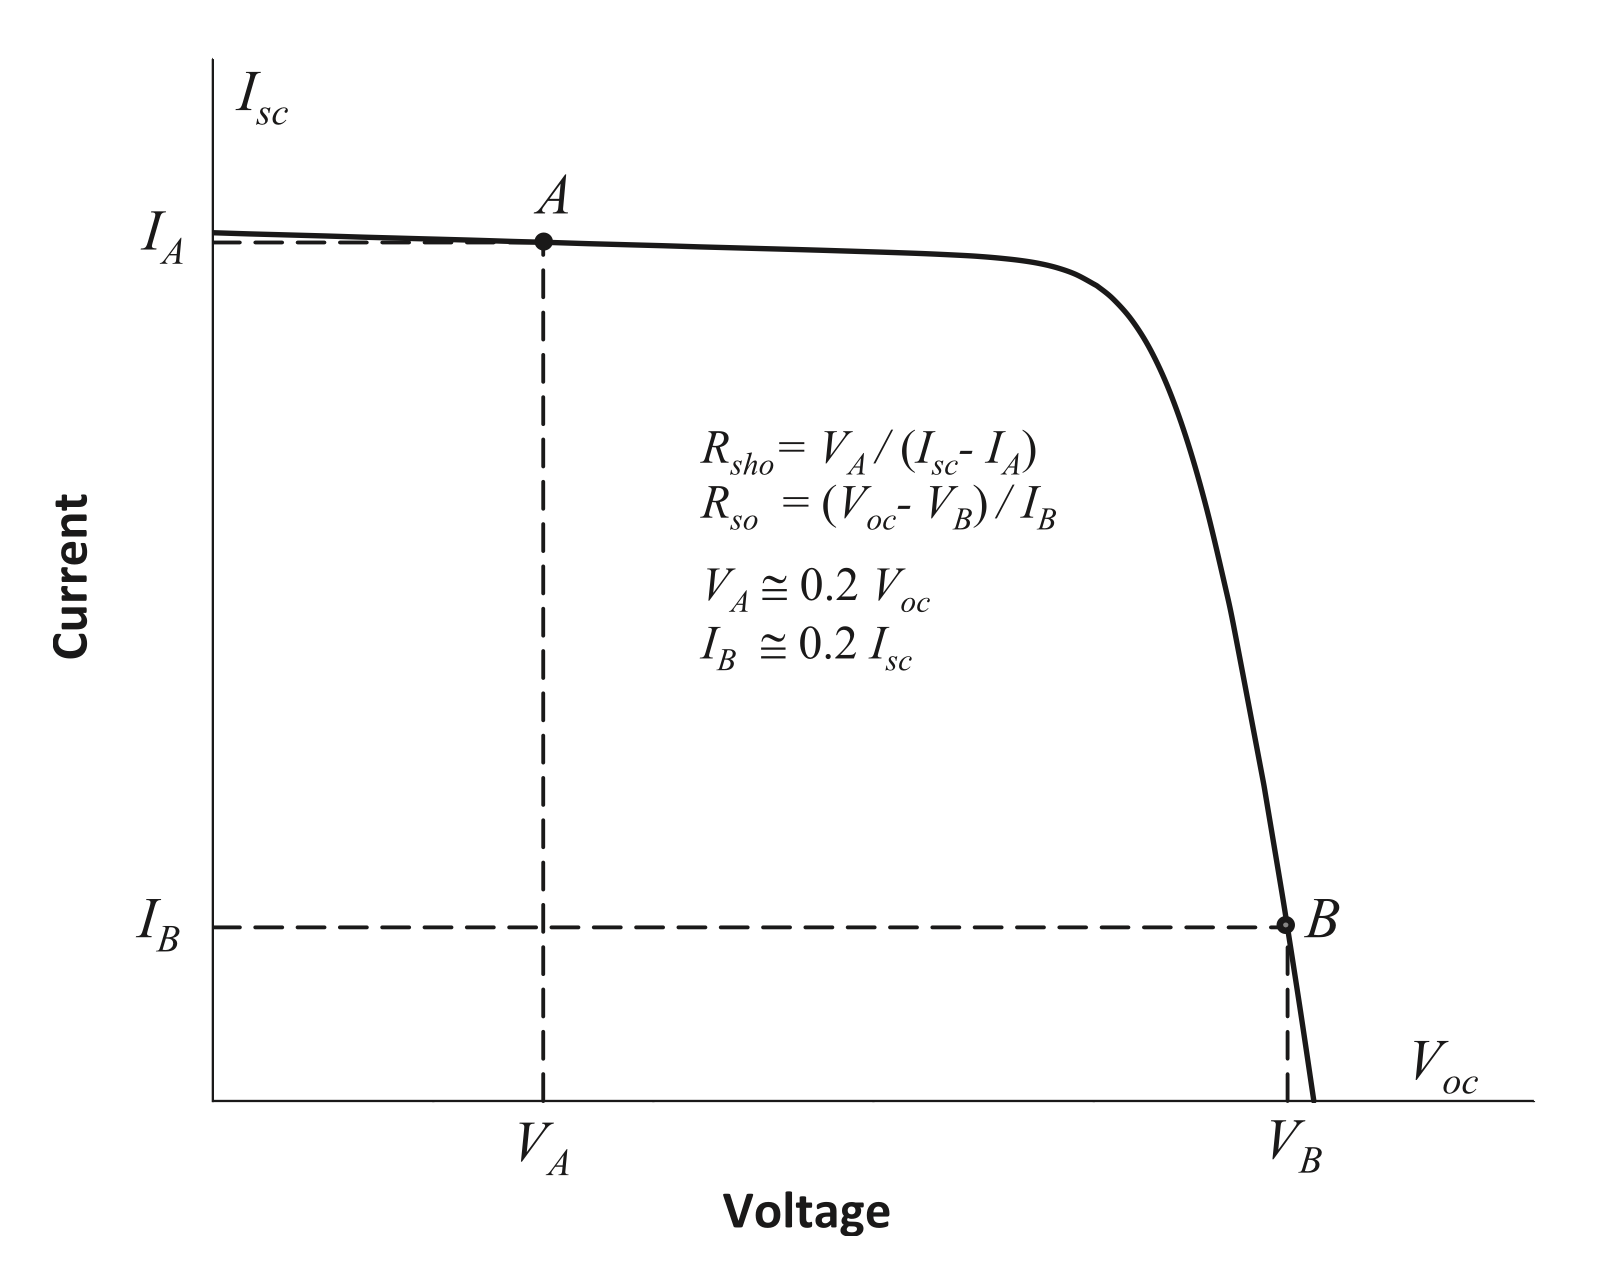
\includegraphics[scale=0.20]{Orioli_estimation_of_Rso_and_Rsho.png}
    \caption{\small Graphical evaluation of \(R_{\text{so}}\) and \(R_{\text{sho}}\) in the I-V characteristic at STC \cite{Orioli}.}
    \label{fig:Orioli_estimation_of_Rso_and_Rsho}
\end{figure}

The solution of Equations \ref{eq:IV_at_short_circuit_point_at_SRC} to
\ref{eq:IV_derivative_at_open_circuit_point_at_SRC} was initially
attempted using software like Mathematica and MATLAB. However, the
authors could not achieve a valid solution and proposed a numerical
algorithm instead, which consists of a double trial-and-error
process with the second nested within the first. The process starts
with an initial guess of \(R_{\text{s}}\) and \(n\), and the following conditions:

\begin{equation}
    I_{\text{L,ref}} = I_{\text{sc,ref}} \qquad R_{\text{sh}} = R_{\text{sho}}
    \label{eq:LoBrano_Orioli_initial_conditions}
\end{equation}

\noindent
These conditions are obtained from Equations \ref{eq:IV_at_short_circuit_point_at_SRC}
and \ref{eq:IV_derivative_at_short_circuit_point_at_SRC} under the commonly satisfied
assumptions \cite[p. 1362]{LoBrano}:

\begin{equation}
    R_{\text{s}} \ll R_{\text{sho}} \qquad \frac{I_{\text{0,ref}}}{nT_{\text{ref}}}\exp\bigl(\frac{I_{\text{sc,ref}}R_{\text{s}}}{nT_{\text{ref}}}\bigr) \ll \frac{1}{R_{\text{sh}}}
\end{equation}

\noindent
The inner trial evaluates \(I_{0}\), \(I_{\text{L}}\), \(R_{\text{sh}}\) and \(n\) in
sequence using Equations \ref{eq:IV_at_maximum_power_point_at_SRC},
\ref{eq:IV_at_short_circuit_point_at_SRC}, \ref{eq:IV_derivative_at_short_circuit_point_at_SRC},
and \ref{eq:IV_at_open_circuit_point_at_SRC} until convergence of n is
achieved with the desired accuracy. The outer trial recalculates \(R_{\text{s}}\)
with Equation \ref{eq:IV_derivative_at_open_circuit_point_at_SRC} after
each inner trial and repeats the process until convergence of \(R_{\text{s}}\) is
achieved with the desired accuracy. In this way, the five equations are
solved in a non-approximate form because no simplifications are used.
It is worth noting that the procedure in \cite[p. 1163f]{Orioli} to determine
the values in step (i) uses the positions in Equation \ref{eq:LoBrano_Orioli_initial_conditions}
as parameters and determines the remaining values \(I_{\text{0,ref}}\), \(n\) and \(R_{\text{s}}\)
in a single trial-and-error process using Equations
\ref{eq:IV_at_open_circuit_point_at_SRC}, \ref{eq:IV_at_maximum_power_point_at_SRC},
and \ref{eq:IV_derivative_at_open_circuit_point_at_SRC}, leading to a satisfactory
approximate set of parameters.

The thermal correction factor K has the effect of shifting the I-V curve at irradiance
\(G_{\text{ref}}\) along the voltage axis to better fit the characteristics provided by the
manufacturer at temperatures \(T^*\) different from \(T_{\text{ref}}\) \cite[p. 1365]{LoBrano}.
The procedure described in \cite{Orioli} is presented, which does not require knowledge
of the maximum power point at a temperature \(T = T^*\) different from \(T_{\text{ref}}\),
unlike the method presented in \cite{LoBrano}. The parameter \(K\) will be determined for
a chosen temperature \(T^*\) such that the corresponding maximum power at reference
irradiance equals the value of the maximum power obtained by:

\begin{equation}
    P_{\text{mp}}^* = P_{\text{mp,ref}} (1 + \frac{\mu_{P_{\text{mp}}}}{100} (T^* - T_{\text{ref}}))
    \label{eq:Maximum_power_in_correspondence_to_temperature_coefficient}
\end{equation}

\noindent
where \(\mu_{P_{\text{mp}}}\) is the temperature coefficient of the
maximum power point provided by the manufacturer. The temperature \(T^*\)
should be chosen by considering the maximum or minimum expected operating
temperature for the PV module \cite[p. 1365]{LoBrano}.
It is evident that the problem of finding the maximum power on the I-V
curve in the described setting can equivalently be formulated as:

\begin{alignat}{2}
    & \max_{V_{\text{d}}, I}    & \quad & V_{\text{d}} I - I^2 [R_{\text{s}} + K(T^* - T_{\text{ref}})]
    \label{eq:Parameter_K_optimization_problem_objective} \\
    & \text{subject to} & \quad & I - I_{\text{L}}^* + I_{0}^* \left[\exp\left(\frac{V_{\text{d}}}{nT^*}\right) - 1\right] + \frac{V_{\text{d}}}{R_{\text{sh}}} = 0
    \label{eq:Parameter_K_optimization_problem_constraint}
\end{alignat}

\noindent
Here, \(I_{\text{L}}^*\) and \(I_{0}^*\) are the photocurrent and reverse saturation current
at the considered operating conditions, and the substitution \(V_{\text{d}} = V + KI(T^* - T_{\text{ref}}) +IR_{\text{s}}\)
represents the voltage across the diode \cite[p. 1166]{Orioli}. Instead of
finding \(K\) through a trial-and-error process, wherein each iteration compares
the calculated maximum power point for the given \(K\) is compared with \(P_{\text{mp}}^*\), the
authors propose a numerical procedure based on the method of Lagrange
multipliers. The idea is to find a Karush-Kuhn-Tucker (KKT) point in
each iteration of the equivalent equality-constrained optimization
problem and compare the corresponding maximum power of the original
problem with \(P_{\text{mp}}^*\)  until convergence of \(K\) is achieved
with the desired accuracy. The Lagrange multiplier rule of the equality
contraint optimization problem takes the form:

\begin{align}
    I + \lambda \Biggl[ \frac{I_{0}^*}{nT} \exp \Biggl( \frac{V_{\text{d}}}{nT^*}\Biggr) + \frac{1}{R_{\text{sh}}}\Biggr] &= 0
    \label{eq:Parameter_K_optimization_problem_multiplier_rule_dVd} \\
    V_{\text{d}} - 2I[R_{\text{s}} + K(T-T_{\text{ref}})] + \lambda &= 0 
    \label{eq:Parameter_K_optimization_problem_multiplier_rule_dI}
\end{align}

\noindent
where \(\lambda\) denotes the Lagrange multiplier.
By expressing \(\lambda\) from Equation \ref{eq:Parameter_K_optimization_problem_multiplier_rule_dI}
and substituting it into Equation \ref{eq:Parameter_K_optimization_problem_multiplier_rule_dVd},
setting the result equal to the constraint in Equation \ref{eq:Parameter_K_optimization_problem_constraint},
and solving for \(V_{\text{d}}\) in the exponential term, the following expression is obtained:

\begin{equation}
    V_{\text{d}} = nT^* \Biggl[ \ln \Biggl( \frac{R_{\text{sh}}(I_{\text{L}}^* + I_{0}^*) - 2(V_{\text{d}} - I\tilde{R}_{\text{s}})}{R_{\text{sh}}(V_{\text{d}} - 2I\tilde{R}_{\text{s}})} \Biggr)- \ln \Biggl( I_{0}^* \Bigl( \frac{1}{nT^*} + \frac{1}{V_{\text{d}} - 2I\tilde{R}_{\text{s}}} \Bigr) \Biggr)\Biggr]
    \label{eq:Parameter_K_optimization_problem_fixpoint}
\end{equation}

\noindent
where \(\tilde{R}_{\text{s}} = R_{\text{s}} + K(T^* - T_{\text{ref}})\). Each inner loop of
finding \(K\) starts by initializing:

\begin{equation}
    V_{\text{d}} = -nT^* \ln\biggl( \frac{I_{0}^*}{nT^*} \biggr)
\end{equation}

\noindent
The procedure iteratively evaluates Equations \ref{eq:Parameter_K_optimization_problem_multiplier_rule_dVd}
and \ref{eq:Parameter_K_optimization_problem_fixpoint} in sequence, for six iterations as
suggested by \cite{Orioli}, to obtain a stable value of \(V_{\text{d}}\), denoted \(V_{\text{d,mp}}\). The
corresponding maximum power of the original problem, needed for comparison with
\(P_{\text{mp}}^{*}\), is derived from the equality constraint
(Equation \ref{eq:Parameter_K_optimization_problem_constraint}) and the substitution:

\begin{align}
    I_{\text{mp}} &= I_{\text{L}}^* - I_{0}^* \left[\exp\left(\frac{V_{\text{d,mp}}}{nT^*}\right) - 1\right] - \frac{V_{\text{d,mp}}}{R_{\text{sh}}} = 0 \\
    V_{\text{mp}} &= V_{\text{d,mp}} - KI(T-T_{\text{ref}}) - IR_{\text{s}}
\end{align}

\noindent
The authors of \cite{Orioli} used the slightly different objective function
\(V_{\text{d}}I - I^2R_{\text{s}}\) in Equation \ref{eq:Parameter_K_optimization_problem_objective},
which does not yield an equivalent problem. Consequently, the above procedure
differs from the one described in their paper. As can be seen from the steps
above, the original procedure uses \(R_{\text{s}}\) instead of \(\tilde{R}_{\text{s}}\) in Equation
\ref{eq:Parameter_K_optimization_problem_fixpoint}. Both
procedures have been compared by applying them to the four investigated PV modules in \cite{Orioli},
using a trial-and-error process in which the maximum power is found through
a nonlinear solver. The results are presented in Table \ref{tab:Parameter_K_procedure_comparision}.
As expected, using the objective function of the equivalent problem leads
to the same values of \(K\), confirmed by a difference of zero in the first
four rows. However, the objective function used in \cite{Orioli} leads to
small deviations, as seen in the last four rows. The authors do not
comment on this. Since the parameter \(K\) is a constant that only needs to
be calculated once, and its computation using a non-linear solver is fast,
this method may be preferred over the presented numerical procedure. 

\begin{table}
    \centering
    \resizebox{\columnwidth}{!}{
        \begin{tabular}{lll}
            \toprule
            Objective function & PV module & Difference in calculated K \\
            \midrule
            \(V_{\text{d}}I - I^2(R_{\text{s}} + K[T^*-T_{\text{ref}}])\) & Gruposolar GS601456P-218 & 0 \\
             & Kyocera KC175GHT-2  & 0 \\
             & Sanyo HIP-230 HDE1 & 0 \\
             & Shell SP75 & 0 \\
            \midrule
            \(V_{\text{d}}I - I^2R_{\text{s}}\) & Gruposolar GS601456P-218 & \(2.17933 \times 10^{-4}\) \\
             & Kyocera KC175GHT-2  & \(3.28 \times 10^{-7}\) \\
             & Sanyo HIP-230 HDE1 & \(2.15202 \times 10^{-4}\) \\
             & Shell SP75 & \(3.58 \times 10^{-6}\) \\
            \bottomrule
        \end{tabular}
    }
    \caption{\small Results of comparision between the procedure of calculating the parameter \(K\) 
             as described in Orioli \cite{Orioli} and the presented procedure based on the 
             equivalent problem.}
    \label{tab:Parameter_K_procedure_comparision}
\end{table}

The first expression to find the parameters of step (ii) is
obtained by evaluating Equation \ref{eq:Orioli_IV_curve_governing_equation}
at the open-circuit point \((V, I) = (0, V_{\text{oc}}(\alpha_{\text{G}}, T))\)
for a given irradiance and temperature:

\begin{equation}
    I_{0}(\alpha_{\text{G}}, T) = \alpha_{\text{G}} \Biggl[ \frac{I_{\text{L}}(T) - \frac{V_{\text{oc}}(\alpha_{\text{G}}, T)}{R_{\text{sh}}}}{\exp \bigl( \frac{V_{\text{oc}}(\alpha_{\text{G}}, T)}{nT}\bigr) - 1 } \Biggr]
    \label{eq:Orioli_photocurrent_Io}
\end{equation}

\noindent
The authors propose the following expression to account for
the dependence of the photocurrent \(I_{\text{L}}(T)\) on temperature:

\begin{equation}
    I_{\text{L}}(T) = I_{\text{L,ref}} + \mu_{\text{I,sc}} \: (T - T_{\text{ref}})
    \label{eq:Orioli_reverse_saturation_current_IL}
\end{equation}

\noindent
where \(\mu_{\text{I,sc}}\) is the short-circuit current temperature coefficient,
which measures the change of short-circuit current values with varying temperature.
To derive a reliable expression for the open-circuit voltage \(V_{\text{oc}}(\alpha_{\text{G}}, T)\)
for monocrystalline, polycrystalline, and Sanyo HIT technology panels, the authors
of \cite{Orioli} collected open-circuit voltage values of 108 PV modules from 23
manufacturers at various irradiance levels and constant temperature \(T_{\text{ref}}\):

\begin{equation}
    V_{\text{oc}}(\alpha_{\text{G}}, T) = V_{\text{oc,ref}}  \: (1 + c_{1}\ln\alpha_{\text{G}} + c_{2}\ln^2\alpha_{\text{G}} + c_{3}\ln^3\alpha_{\text{G}}) + \mu_{\text{V,oc}} (T - T_{\text{ref}})
\end{equation}

\noindent
where \(c_{1} = 5.468511 \times 10^{-2}\), \(c_{2} = 5.973869 \times 10^{-3}\),  
\(c_{3} = 7.616178 \times 10^{-4}\) and \(\mu_{\text{V,oc}}\) is the open-circuit voltage
temperature coefficient, which measures the change of open-circuit voltage
values with varying temperature, analogous to \(\mu_{\text{I,sc}}\) for current.
The constants \(c_{i}\) can be fitted to a specific PV module if open-circuit
voltage values at different irradiance levels are available, which can
sometimes be extracted from graphical data in the datasheet.
The reverse saturation current \(I_{0}(\alpha_{\text{G}}, T)\) for PV panels with
different manufacturing characteristics can be obtained using the
following interpolating equation \cite[p. 1365]{LoBrano}:

\begin{equation}
    I_{0}(\alpha_{\text{G}}, T) = \exp \Biggl[ \Biggl( \frac{\alpha_{\text{G}} - 0.2}{1 - 0.2} \Biggr) \ln \frac{I_{0}(1, T)}{I_{0}(0.2, T)} + \ln I_{0}(0.2, T) \Biggr]
\end{equation}

\noindent
where \(I_{0}(1,T)\) and \(I_{0}(0.2,T)\) are evaluated using Equation
\ref{eq:Orioli_photocurrent_Io} with \(I_{\text{L}}(T)\) as
in Equation \ref{eq:Orioli_reverse_saturation_current_IL}, and:

\begin{align}
    V_{\text{oc}}(1, T)   &= V_{\text{oc,ref}} + \mu_{\text{V,oc}} (T - T_{\text{ref}})     \\
    V_{\text{oc}}(0.2, T) &= V_{\text{oc}}(0.2,25) + \mu_{\text{V,oc}} (T - T_{\text{ref}})
\end{align}

\noindent
Here, \(V_{\text{oc}}(0.2,25)\) denotes the open-circuit voltage at \(G_{\text{c}} = 200 \, \si{\watt\per\square\meter}\)  and
\(T = T_{\text{ref}}\).